% Three consecutive ticks of the same selector tree. For each tick we
% number the evaluation order above each visited child, colour by
% status (green = success, red = failure, orange = running), and
% grey out children that were skipped by short-circuit evaluation.
\documentclass[border=6pt,tikz]{standalone}
\usepackage{tikz}
\usepackage{amsmath, amssymb}
\usepackage[T1]{fontenc}
\usepackage{lmodern}
\usetikzlibrary{arrows.meta, positioning, fit, shapes.geometric, backgrounds}

\tikzset{
  composite/.style = {draw, rounded corners=2pt, fill=blue!10, align=center,
                      font=\small\bfseries, inner sep=3pt,
                      minimum width=1.4cm, minimum height=0.7cm},
  condition/.style = {draw, ellipse, align=center, font=\scriptsize,
                      inner sep=3pt, minimum width=1.6cm, minimum height=0.75cm},
  action/.style    = {draw, rectangle, align=center, font=\scriptsize,
                      inner sep=3pt, minimum width=1.6cm, minimum height=0.75cm},
  % status overlays: only override fill
  neutral/.style   = {fill=yellow!18},
  neutralA/.style  = {fill=green!16},
  unvisited/.style = {fill=black!5, text=black!35, draw=black!30},
  statusS/.style   = {fill=green!45, draw=black!75},
  statusF/.style   = {fill=red!30,   draw=black!75},
  statusR/.style   = {fill=orange!40, draw=black!75},
  % evaluation-order tag
  ordertag/.style  = {font=\tiny\bfseries, text=purple!70!black,
                      fill=white, inner sep=1pt, rounded corners=1pt,
                      draw=purple!70!black, line width=0.3pt},
  flow/.style      = {-, line width=0.55pt},
  solidflow/.style = {-, line width=0.7pt, black!80},
  skipflow/.style  = {-, line width=0.55pt, dashed, black!30},
  title/.style     = {font=\small\bfseries, text=black!80, align=center},
  caption/.style   = {font=\scriptsize, text=black!75, align=center,
                      text width=4.2cm},
  rootlabel/.style = {font=\tiny\bfseries, align=center},
  group/.style     = {draw=black!25, rounded corners=6pt, fill=black!3,
                      inner sep=11pt, line width=0.5pt},
}

% Draw one panel.
%   #1: panel name prefix
%   #2: caption
%   #3/#4/#5: style-override for children 1..3 (pass e.g. statusF or unvisited)
%   #6/#7/#8: order-tag text for each visited child (empty = none)
%   #9: root status line (SUCCESS / FAILURE / RUNNING)
\newcommand{\tickpanel}[9]{%
  \node[composite]                                              (#1R) {$?$\\[-1pt]\scriptsize root};
  \node[condition, neutral,  #3, below left=0.7cm and 0.1cm of #1R] (#1A) {$c_{hungry}$};
  \node[condition, neutral,  #4, below=0.75cm of #1R]               (#1B) {$c_{battery}$};
  \node[action,    neutralA, #5, below right=0.7cm and 0.1cm of #1R](#1C) {$a_{eat}$};
  \ifx&#6&\else\node[ordertag, above=-1pt of #1A.north east] {#6};\fi
  \ifx&#7&\else\node[ordertag, above=-1pt of #1B.north east] {#7};\fi
  \ifx&#8&\else\node[ordertag, above=-1pt of #1C.north east] {#8};\fi
  \draw[flow] (#1R) -- (#1A);
  \draw[flow] (#1R) -- (#1B);
  \draw[flow] (#1R) -- (#1C);
  \node[caption, below=1.0cm of #1B] (#1cap) {#2};
  \node[font=\scriptsize\bfseries, below=3pt of #1cap.south]
    (#1root) {root $=$ #9};
  \begin{scope}[on background layer]
    \node[group, fit=(#1R)(#1A)(#1C)(#1cap)(#1root)] (#1g) {};
  \end{scope}
}

\begin{document}
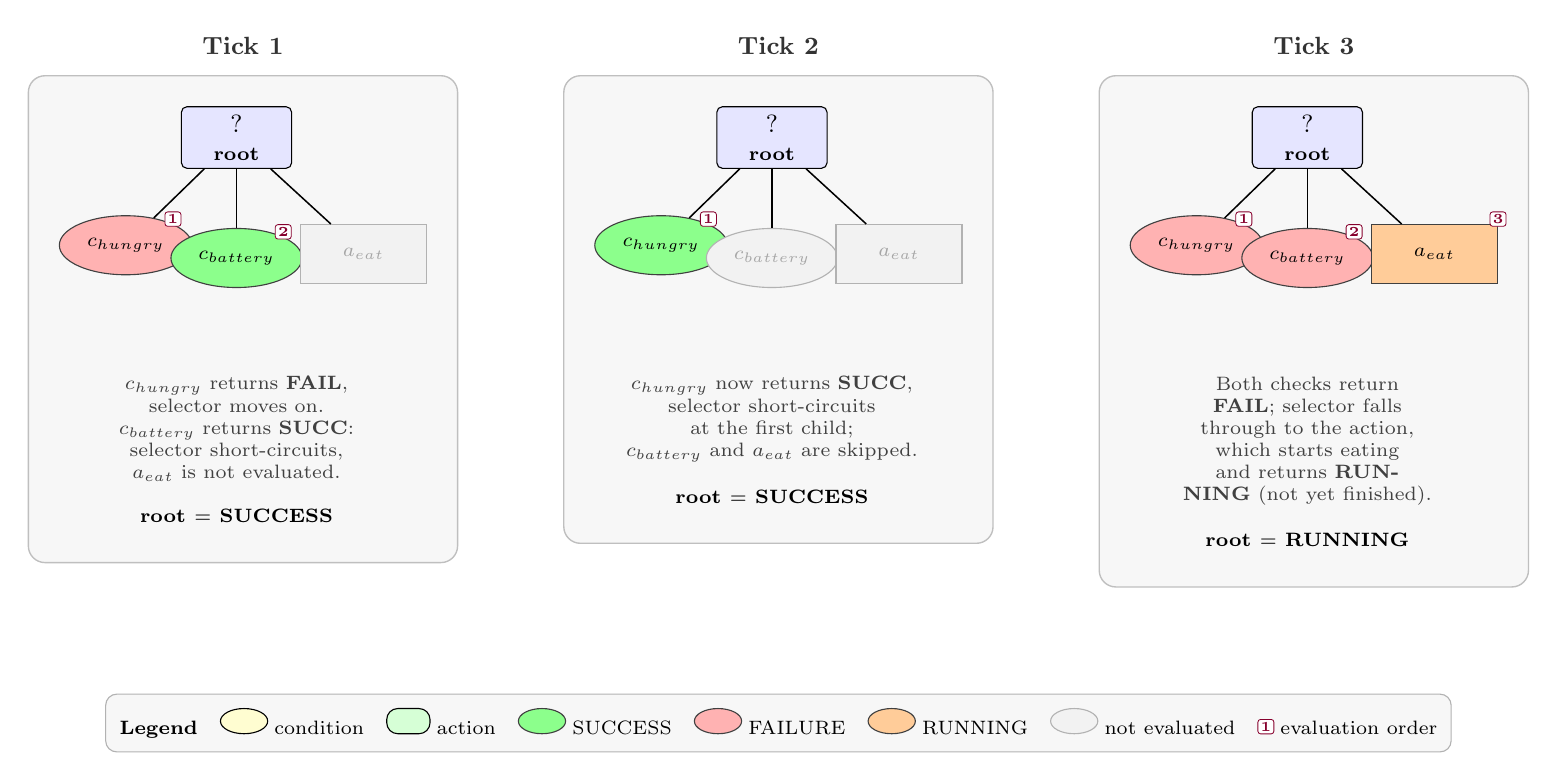
\begin{tikzpicture}

% ===== Tick 1: hungry FAIL, battery SUCC (short-circuits) =====
\tickpanel{t1}{%
  $c_{hungry}$ returns \textbf{FAIL}, selector moves on.\\
  $c_{battery}$ returns \textbf{SUCC}: selector short-circuits,\\
  $a_{eat}$ is not evaluated.}
  {statusF}{statusS}{unvisited}
  {1}{2}{}
  {SUCCESS}
\node[title, above=4pt of t1g.north] {Tick 1};

% ===== Tick 2: hungry SUCC (short-circuits immediately) =====
\begin{scope}[shift={(6.8cm,0)}]
\tickpanel{t2}{%
  $c_{hungry}$ now returns \textbf{SUCC},\\
  selector short-circuits at the first child;\\
  $c_{battery}$ and $a_{eat}$ are skipped.}
  {statusS}{unvisited}{unvisited}
  {1}{}{}
  {SUCCESS}
\node[title, above=4pt of t2g.north] {Tick 2};
\end{scope}

% ===== Tick 3: both checks FAIL; action returns RUNNING =====
\begin{scope}[shift={(13.6cm,0)}]
\tickpanel{t3}{%
  Both checks return \textbf{FAIL}; selector falls\\
  through to the action, which starts eating\\
  and returns \textbf{RUNNING} (not yet finished).}
  {statusF}{statusF}{statusR}
  {1}{2}{3}
  {RUNNING}
\node[title, above=4pt of t3g.north] {Tick 3};
\end{scope}

% ===== Legend =====
\node[draw=black!30, rounded corners=4pt, fill=black!3,
      align=left, font=\scriptsize, inner sep=5pt,
      below=1.9cm of t2g.south]
  (legend)
  {\textbf{Legend}\quad
   \tikz\node[condition,minimum width=0.6cm,minimum height=0.32cm,inner sep=0pt,font=\tiny,fill=yellow!18]{};\;condition\quad
   \tikz\node[action,minimum width=0.55cm,minimum height=0.32cm,inner sep=0pt,font=\tiny,fill=green!16]{};\;action\quad
   \tikz\node[condition,statusS,minimum width=0.6cm,minimum height=0.32cm,inner sep=0pt,font=\tiny]{};\;SUCCESS\quad
   \tikz\node[condition,statusF,minimum width=0.6cm,minimum height=0.32cm,inner sep=0pt,font=\tiny]{};\;FAILURE\quad
   \tikz\node[condition,statusR,minimum width=0.6cm,minimum height=0.32cm,inner sep=0pt,font=\tiny]{};\;RUNNING\quad
   \tikz\node[condition,unvisited,minimum width=0.6cm,minimum height=0.32cm,inner sep=0pt,font=\tiny]{};\;not evaluated\quad
   \tikz\node[ordertag, inner sep=1pt, font=\tiny\bfseries]{1};\;evaluation order};

\end{tikzpicture}
\end{document}
